% Chapter 5

\chapter{Experiments} % Main chapter title

\label{Chapter5} % For referencing the chapter elsewhere, use \ref{Chapter4} 

%----------------------------------------------------------------------------------------

The two-dimensional Branin-Hoo function is often used as a bench-mark for optimization \cite{eggensperger2013towards} \cite{picheny2013benchmark}. For our experiments, we use a deterministic version \cite{sfu} rescaled to the unit square $[0,1]^2$ with
%
\begin{equation} \label{eq:branin}
f(\x) = \frac{1}{51.95} \left[ (\bar{x}_2 - \frac{5.1}{4\pi^2}\bar{x}_1^2 + \frac{5}{\pi}\bar{x}_1 - 6)^2 + 10(1-\frac{1}{8\pi}\cos(\bar{x}_1)) - 44.81 \right] 
\end{equation} 
%
where $\bar{x}_1 = 15x_1 - 5$ and $\bar{x}_2 = 15x_2$. This rescaled version has mean zero and variance one. It is a multi-modal function with global minima $-1.047$ at three locations: $(0.124, 0.818)$, $(0.543, 0.152)$ and $(0.962, 0.165)$, to three decimal places.

\section{Unconstrained} \label{experiment1}

To demonstrate the capability of Bayesian optimization we first optimize the unconstrained Branin-Hoo function. 

The optimization budget is taken to be $N = 20$ function evaluations. An initial dataset $\Da_0$ of five points is generated by latin-hypercube sampling (LHS), leaving fifteen iterations to be selected by the chosen acquisition function.

\begin{figure}
\centering
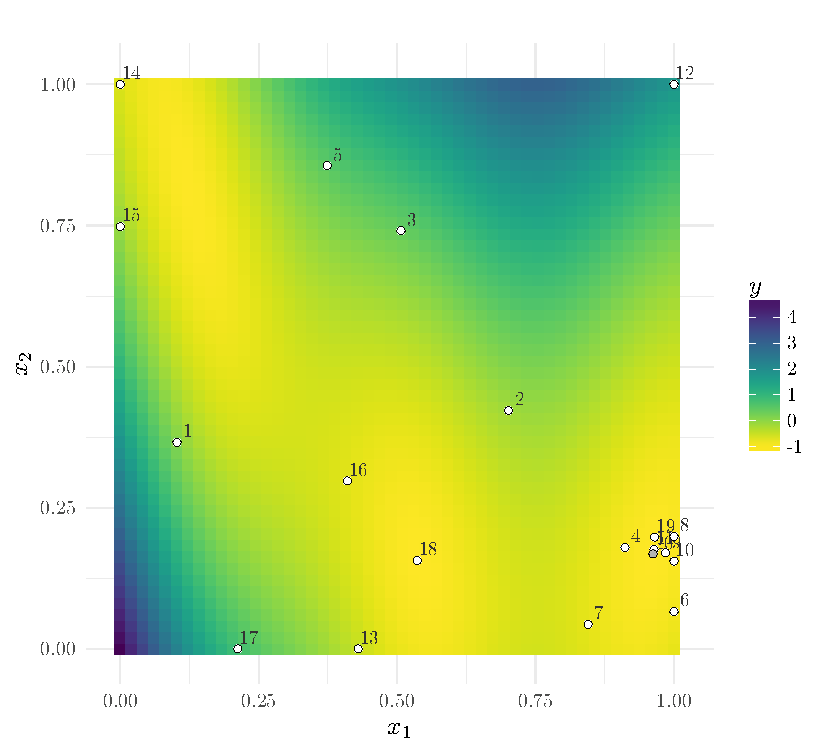
\includegraphics[scale=1]{fig5i.pdf}
\caption{Density plot of modified Branin-Hoo function, as specified by equation \ref{eq:branin}. Example numbered Bayesian optimization path plotted as white circles. Points one to five are generated by latin-hypercube sampling and points six to twenty are chosen by maximizing EI acquisition function. Minimum sample location, shown as the grey circle, is the final point $(0.965, 0.198)$ with value $-1.043$ to three decimal places.} \label{fig:5i}
\end{figure}

The implementation of is written in R using the \texttt{laGP} \cite{gramacy2016lagp} package, based on the lecture notes of \citet{lectures}. For simplicity an isotropic squared exponential kernel is used. To ease computation the prior mean function $\mu_0$ of the GP is set to be zero and the amplitude $\sigma_f^2$ of the kernel is set to be one. The length-scale $l$ of the kernel is tuned at each iteration of the algorithm to be the maximum likelihood estimator. The acquisition function used is expected improvement with incumbent value $\nu$ set to be the minimum function value observed so far. One benefit of choosing EI is that it does not require any additional parameters, such as the constant $\lambda$ for LCB. Both the optimization of the log-likelihood, given by equation \ref{eq:loglike}, and the optimization of the acquisition function are performed using five random restarts of \texttt{method="L-BFGS-B"} via the default function \texttt{optim}.

\begin{figure}
\centering
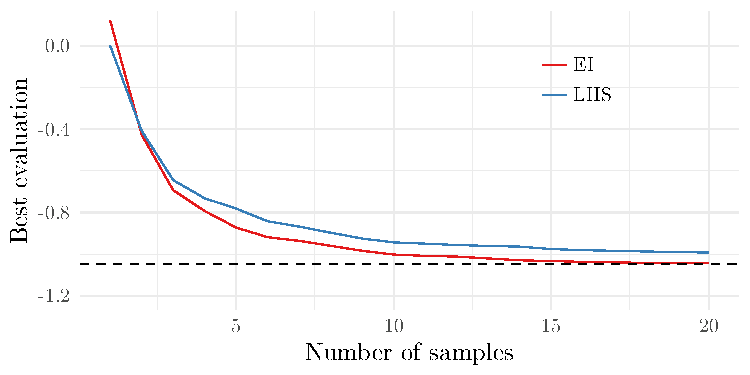
\includegraphics[scale=1]{fig5ii.pdf}
\caption{The progress, averaged over 50 runs, of both EI and LHS. Recall that the first five points chosen by both methods are by LHS, so the variation for these samples is due to randomness. However from that point onwards it is clear that EI convincingly converges on the true global minimum -1.047, shown by the horizontal dashed line, whereas LHS makes comparatively slow progress.} \label{fig:5ii}
\end{figure}

Figure \ref{fig:5i} shows the result of one run of the Bayesian optimization procedure, which we henceforth refer to as EI, described above. Of course the results of any single run are not statistically significant because the first five samples locations, together with the starting locations of the log-likelihood and acquisition function optimization procedures, are random.  

To average out some of the variation we repeat the EI procedure independently 50 times. To provide a baseline for comparison we also run 50 repeats where all 20 points are chosen by LHS. Figure \ref{fig:5ii} compares the average performance of each procedure. It is clear that the performance of EI in this instance is superior: 29 out of the 50 times EI finds a global minimum to three decimal places compared to only once out of 50 for LHS. 

\section{Constrained} \label{experiment2}

Similarly to the set-up in \citet{gelbart} and Griffiths \cite{griffiths} we now consider as before the optimization the Branin-Hoo function, but now with the additional, deterministic, black-box disk constraint $c(\x) \geq 0$, where:
%
\begin{equation}
c(\x) = \frac{2}{9} - (x_1 - \frac{1}{2})^2 - (x_2 - \frac{1}{2})^2
\end{equation}
%
This constraint excludes points outside a circle of radius $\sqrt{2}/3$ centred at $(0.5, 0.5)$. Of the three global minimizers of the unconstrained objective function, two now lie outside the feasible region, leaving only one feasible global minimizer, $(0.543, 0.152)$. It is assumed that the constraint is coupled, so that $f$ and $c$ are evaluated jointly.

We will test the performance of the two constrained optimization acquisition functions introduced in Chapter \ref{Chapter4}, EIC and constrained IECI, together with LHS. As before, the optimization budget is $N=20$ and the first five iterations of each method are chosen by LHS. 

In both the EIC and IECI implementations the constraint, like the objective function, is modelled by a GP with squared exponential kernel and the incumbent value $\nu$ is set to be the minimum function value observed so far. Whereas EIC is entirely tractable, the integral in IECI is approximated by a sum weighted by the probability of satisfying the constraint. For this reason IECI was substantially more computationally demanding.

Figure \ref{fig:5iii} illustrates the region which is now infeasible due to the constraint and shows an example EIC optimization path. Figure \ref{fig:5iv} shows the surrogate functions to the objective and constraint functions, respectively, after the 20 points in the previous figure have been sampled. In this specific instance it is clear that the surrogates are well fitted to both the objective and constraint.

Overall, across 50 repeats, we find that EIC performs slightly better than IECI, with both performing much better than LHS. In particular, the average of the minimum feasible function evaluations found is -1.037 for EIC, -1.032 for IECI and -0.966 for LHS. This is shown by figures \ref{fig:5v} and \ref{fig:5vi}. 

\begin{figure}
\centering
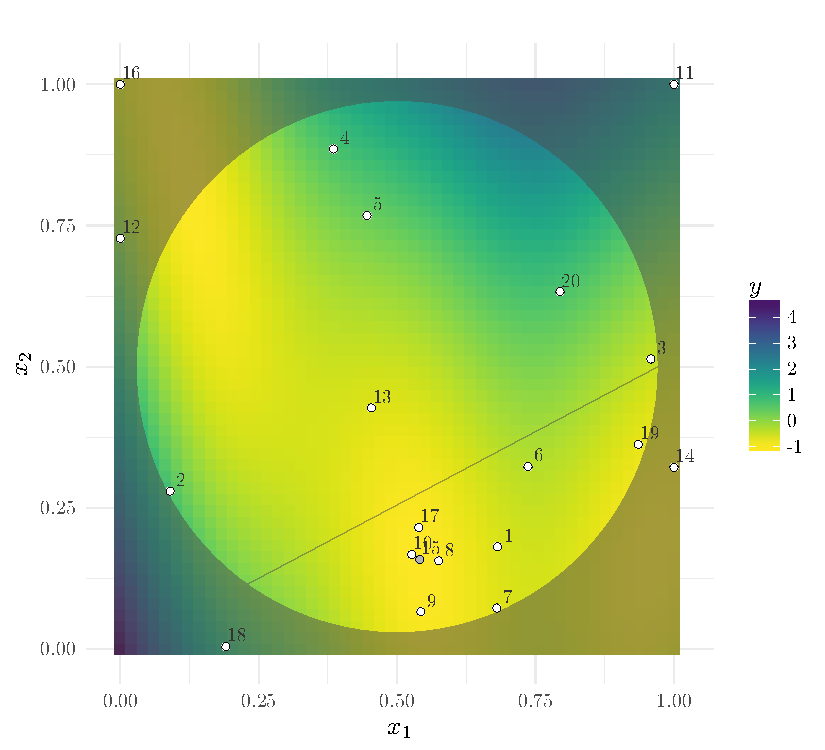
\includegraphics[scale=1]{fig5iii.pdf}
\caption{As in figure \ref{fig:5i} a density plot of Branin-Hoo function is shown. The region which is infeasible, that is $c(\x) < 0$, is shaded in a darker colour. The white circles show a numbered example EIC optimization path, with the grey circle showing minimum feasible sample location $(0.541, 0.158)$ with value -1.047 to three decimal places. In this instance EIC is able to find the one feasible global minimizer. It is interesting to note samples 11, 12, 14, 16 and 18 are taken close to the edge of the unit square.} \label{fig:5iii}
\end{figure}

\begin{figure}
\centering
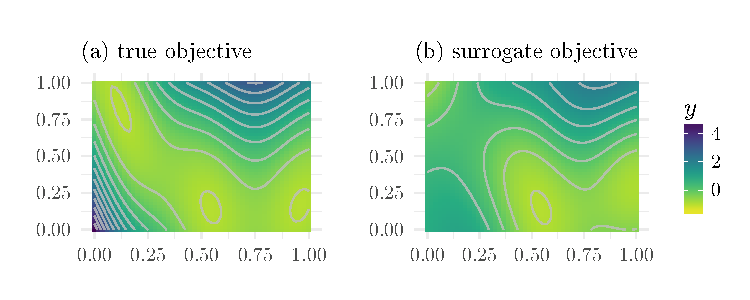
\includegraphics[scale=1]{fig5iva.pdf}

\vspace{-20pt}

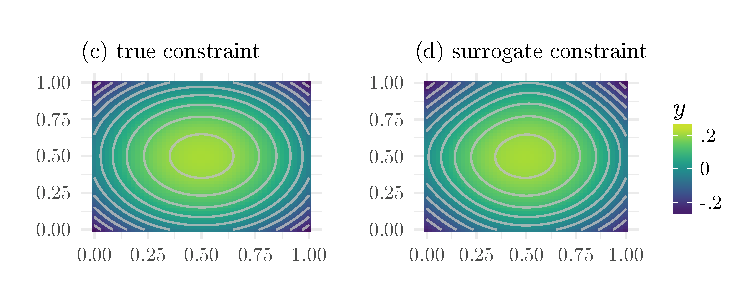
\includegraphics[scale=1]{fig5ivb.pdf}
\caption{
Plots (a) and (b) show the true objective function and the mean of its GP emulator after the 20 points in figure \ref{fig:5iii} have been sampled. To allow for meaningful comparison, they have been rescaled to a common colour scale. Although the surrogate is overall a good fit, it misses the minimizer in the top left. This corresponds to the fact that there are no samples in that location in figure \ref{fig:5iii}. It is also instructive to note that the surrogate function does not fit well in regions where the objective function is high, and that this is not a bad thing. We are only interested in accurately learning the objective function in regions where it may plausibly have a global minimizer.
% 
Similarly, plots (c) and (d) show the true constraint function and the mean of its GP emulator after the 20 samples in figure \ref{fig:5iii}, on a common colour scale (which is oppositely oriented, because we are looking for positive constraint values). The surrogate is very similar to the true constraint, perhaps due to the constraints simplicity.} 
\label{fig:5iv}
\end{figure}

\begin{figure}
\centering
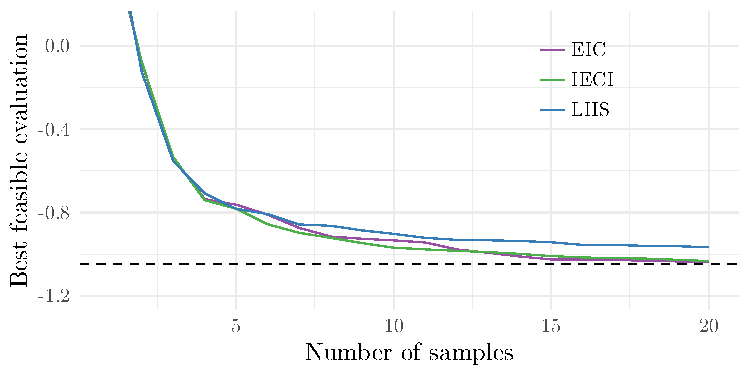
\includegraphics[scale=1]{fig5v.pdf}
\caption{The progress, averaged over 50 runs, of the EIC, IECI and LHS implementations. As in figure \ref{fig:5ii} the true global minimum -1.047 is shown by the horizontal dashed line.} 
\label{fig:5v}
\end{figure}

\begin{figure}
\centering
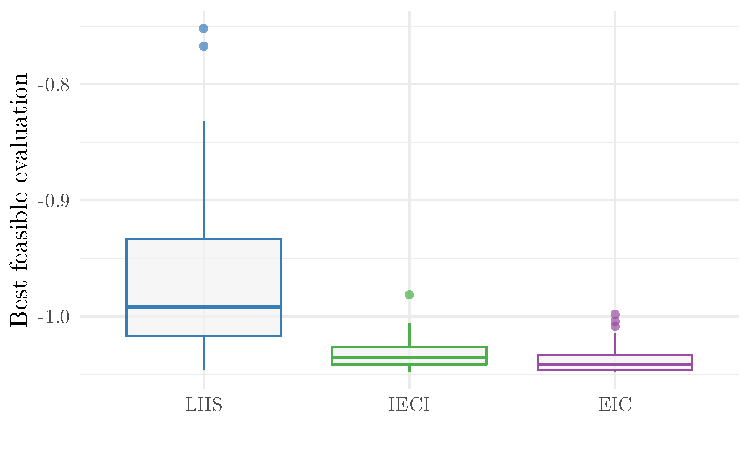
\includegraphics[scale=1]{fig5vi.pdf}
\caption{Boxplot of the best feasible evaluation found after 20 samples for each method, across the 50 runs.} 
\label{fig:5vi}
\end{figure}

One explanation for why EIC may have outperformed IECI in this particular problem is because of the simplicity of the constraint. In particular, there is not much that can be learned from sampling in the infeasible region as the global minimizer is a fair distance from it. Perhaps IECI may prove its value for problems with more complicated feasible regions. Another explanation is that the IECI implementation is only an approximation: it may be that the true version would perform better. This is plausible because a previous implementation of IECI was run with a faster, less accurate, approximation which averaged only -1.017.

\section{Discussion}

These results show the promise of Bayesian optimization and that the algorithm works essentially as hoped, for both unconstrained and unconstrained optimization problems. Of course from a critical point of view there are some caveats which should be mentioned. 

Firstly, in both the constrained and unconstrained cases, the Bayesian optimization implementations are in some sense unfairly helped by the objective function being scaled to have mean zero and variance one, as they have not had to learn these facts from the data.

The Branin-Hoo function is not a particularly difficult optimization problem. As all of the local minimizers are global so there is no threat of placing too great an emphasis on local search. That being said, there is circumstantial evidence of a balanced approach in figures \ref{fig:5i} and \ref{fig:5iii}. Furthermore, it is only two-dimensional which, while being convenient for visualisation, is not particularly demanding. One current challenge is scaling Bayesian optimization to be more effective in higher dimensions, as for the time being it is restricted to roughly 10 dimensions \cite{wang2016practical}.

Furthermore, both the objective and constraint are taken to be deterministic. Had property \ref{itm:p4} been the case the results surely would have been less impressive. Problems with high noise-levels are particularly challenging and can lead to odd, pathological, behaviour if not considered more thoroughly \cite{gelbart} \cite{letham2017constrained}.

Finally, it almost goes without saying that we have only tested performance on one specific function - more rigorous benchmarks should test on a variety of objective functions.





